\documentclass{article}
\usepackage{xeCJK,amsmath,geometry,float,graphicx,amssymb,zhnumber,booktabs,setspace,tasks,verbatim,amsthm,amsfonts,mathdots}
\usepackage{listings,xcolor}
\geometry{a4paper,scale=0.8}   
\title{图论作业 (第八周)}
\author{PB20000113孔浩宇}
\begin{document}
\maketitle
\section*{Ch4}
\subsection*{1.}
    \begin{proof}
        \begin{enumerate}
            \item []
            \item [(1)]$K_5 -e$中四个顶点度为4,一个顶点度为3,无法收缩为顶点度均为4的$K_5$和顶点度均为3的$K_{3,3}$.
            \item [(2)]$K_{3,3} -e$中五个顶点度为3,一个顶点度为2,无法收缩为顶点度均为4的$K_5$和顶点度均为3的$K_{3,3}$.
        \end{enumerate}
        即证.
    \end{proof}

\subsection*{4.}
    \[
        \phi =2-\nu+\varepsilon=2-8+\displaystyle{\frac{8\times 4}{2}}=10.
    \]

\subsection*{6.}
    \begin{enumerate}
        \item [(1)]
            \begin{proof}
                取$G$的任意连通片$G_1$,记$\phi(G_1)=\phi_1,\ \nu(G_1)=\nu_1,\ \varepsilon(G_1)=\varepsilon_1$.
                \[
                    \begin{cases}
                        \ \nu_1 - \varepsilon_1 + \phi_1 &= 2\\
                        \ \qquad\qquad \phi_1 &< 12
                    \end{cases}
                    \ \Rightarrow\ 
                    \nu_1 > \varepsilon_1 -10
                    \xrightarrow{2\varepsilon_1 = \sum \deg(v) \geq 3\nu_1\\}
                    \varepsilon_1 <30.    
                \]
                \[
                    \mbox{if}\ \forall\ f\in G_1,\ \deg(f)\geq 5
                    \ \Rightarrow\ 2\varepsilon_1 \geq 5\phi_1 = 60
                    \ \Rightarrow \varepsilon_1 \geq 30,
                \]
            \end{proof}
            矛盾,即证$\exists\ f\in G,\ \deg(f)\leq 4$.
        \item [(2)]如图.
        \begin{figure*}[htbp]
            \centering
            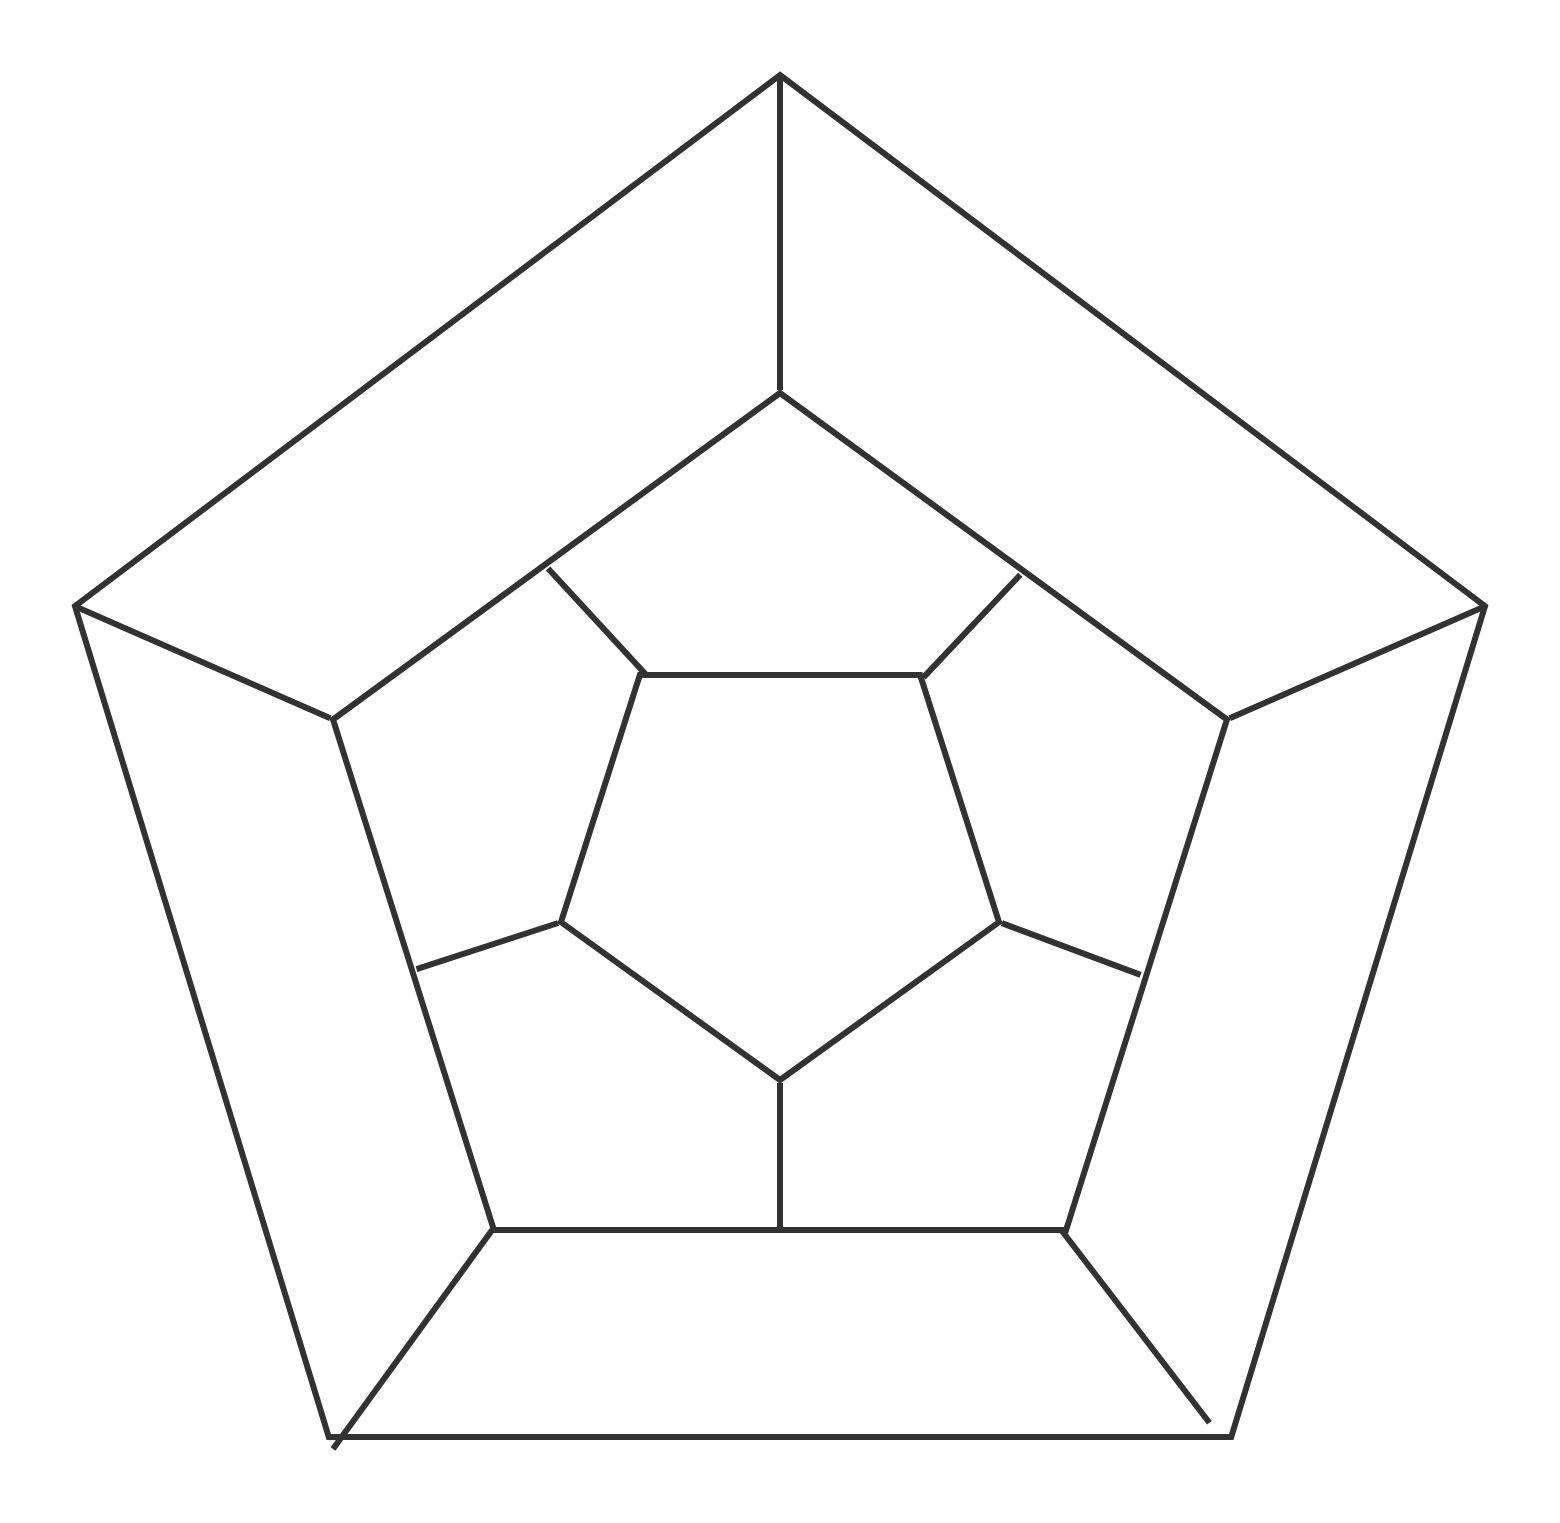
\includegraphics[scale=0.1]{t6.png}
        \end{figure*}
    \end{enumerate}
\clearpage
\subsection*{7.}
\begin{proof}
    \begin{enumerate}
        \item []
        \item [(1)]$\nu \leq 5$,显然成立.
        \item [(2)]$\nu \geq 6$.假设$\delta \geq 5$.
        \[
            \begin{cases}
                \ 2\varepsilon &\geq 5\nu\\
                \ \varepsilon & \leq 3\nu -6
            \end{cases}
            \ \Rightarrow\ 
            \nu \geq 12
            \ \Rightarrow\ 
            \varepsilon \geq \displaystyle{\frac{5\nu}{2}}=30.
        \]
        矛盾,即证$\delta \leq 4$,即$\exists\ v\in V(G),\ \deg(v)\leq 4$.
    \end{enumerate}
\end{proof}

\section*{Ch5}
\subsection*{2.}
\begin{proof}
    假设存在两个不同的完备匹配$M_1$和$M_2$,则$\exists\ u\in G,\ u p_0 \in M_1,\ u q_0 \in M_2(p_0 \neq q_0)$.
    \begin{enumerate}
        \item [(1)]$\exists\ p_0 q_1 \in M_2,\ q_0 p_1 \in M_1$,若$p_1 = q_1$,则$u p_0 q_1 q_0 u$构成圈,与树矛盾。
        \item [(2)]若$p_1\neq q_1$,则$\exists\ p_1 q_2\in M_2,\ q_1 p_2\in M_1$.以此类推,若$\exists\ p_i=q_j$,则
        \[
            \begin{cases}
                u p_0 q_1 \cdots p_i q_j p_{j-1}\cdots q_0 u &(i,j=2k)\\
                \\
                u p_0 q_1 \cdots q_j p_i q_{i-1}\cdots q_0 u &(i,j=2k+1)\\
                \\
                q_j p_{j+1}\cdots p_{i} q_{j} &(j-i=2k+1,j>i)\\
                \\
                p_i q_{i+1}\cdots q_{j} p_{i} &(i-j=2k+1,i>j)
            \end{cases}
        \]
        又$G$存在完备匹配,则$\nu=2k$,总会有$p_i=q_j$.即证矛盾,树至多存在一个完备匹配。
    \end{enumerate}
\end{proof}

\subsection*{4.}
\begin{proof}
    \begin{enumerate}
        \item []
        \item [(1)]$\Rightarrow$:假设$G$中有完备匹配$M$.
        
        记第一个人第i次选的为$p_i$,每选出一个$p_i$,第二个人均可找到$q_i$,使得$p_i q_i\in M$.
        无论如何取$p_i$,总有$q_i$与之相对应,故第二个人有必胜策略。即证当第一个人有必胜策略时,$G$中无完备匹配。
        \item [(2)]$\Leftarrow$:假设$G$中没有完备匹配,最大匹配为$M$.
        
        取$p_1\notin E(M)$,若$\exists\ q_1\notin E(M),\ p_1 q_1\in E(G)$,则$p_1 q_1\in M$,矛盾。
        故$q_1\in E(M)$,则此时等价于以$M$对应的子图为图,原来的第二个人首次选,则原来的第一个人有必胜策略 (见上一问)。

        即证当$G$中无完备匹配时,第一个人有必胜策略。
    \end{enumerate}
\end{proof}
\clearpage
\subsection*{6.}
如图,将正方形方格用红黄相间覆盖,不妨设去除的两个对角为黄色(必同色)。
\begin{figure*}[htbp]
    \centering
    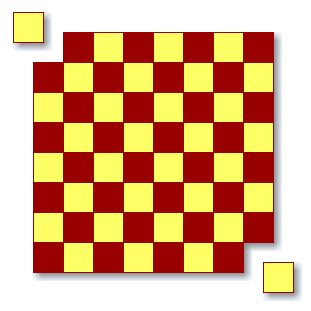
\includegraphics[scale=0.3]{t62.png}
\end{figure*}

将每个格视为一个点,取$E=\{pq|\ p,q\mbox{在图中相邻} \}$,
\[
    X=\{p|\ p\mbox{在黄色格子}\},\ Y=\{q|\ q\mbox{在红色格子} \}.
\]
则$X,\ Y$为图的一个二分划分。由于$|N(Y)|=|X|<|Y|$,故不存在完备匹配。即证不能覆盖。

\subsection*{7.}
\begin{proof}
    \begin{enumerate}
        \item []记$V(G)=X\cup Y,\ X\cap Y=\phi,\ S_X=S\cap X,\ S_Y=S\cap Y$.
        \item [(1)]$\Rightarrow$:
        \begin{align*}
            \mbox{二分图}G \mbox{有完备匹配}
            \Rightarrow\ 
            &X,Y\mbox{中的顶点均被许配}\\
            \Rightarrow\ 
            &|N(S_X)|\geq |S_X|,\ |N(S_Y)|\geq |S_Y|\\
            \Rightarrow\ 
            &|N(S)|=|N(S_X)|+|N(S_Y)|\geq |S_X|+ |S_Y|=|S|.
        \end{align*}
        \item [(2)]$\Leftarrow$:
        \[
            \begin{cases}
                \ |X|\geq |N(X)|&\geq |Y|\\
                \\
                \ |Y|\geq |N(Y)|&\geq |X|
            \end{cases}
            \ \Rightarrow\ 
            \begin{cases}
                \ \ |X| &=|Y|\\
                \\
                \ N(X) &=Y \\
                \\
                \ N(Y) &=X 
            \end{cases}
            \ \Rightarrow\ 
            G\mbox{中存在将$X$的点与$Y$的点一一相配的完备匹配。}
        \]
        \item [(3)]对一般图不成立,如$K_3$满足$\forall\ S\subseteq V(K_3),\ |N(S)|\geq |S|$,但没有完备匹配。
    \end{enumerate}
\end{proof}

\end{document}